\section{Implementation}
\label{sec:sec_algorithm}
\subsection{Architecture of Distributed Video Processing}

\subsubsection{Distributed Video Processing Software Stack}
Figure~\ref{fig:stack} shows the software stack for distributed video
processing.Similar to other types of big data application, data are also stored
in distributed file system such as Google File System (GFS)\cite{gfs}, Hadoop
Distributed File System (HDFS)\cite{hdfs}. However, storing video are more
challenged than storing text because its special structure does not allow
arbitrary partition and requires us to read sequentially.
\begin{figure}[htbp!]\centering
\vspace{-1ex}
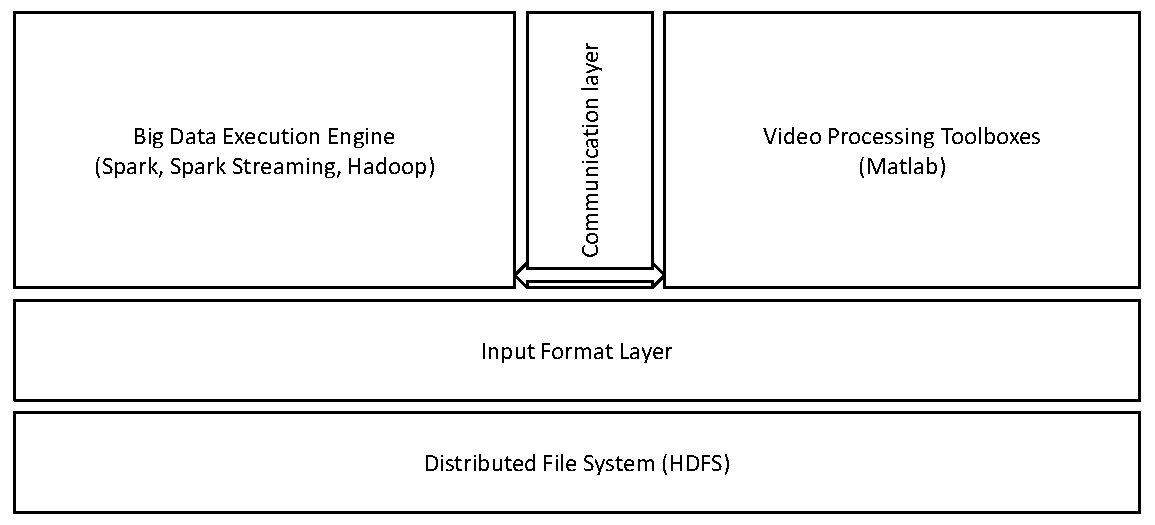
\includegraphics[width=0.5\textwidth]{figures/softwarestack.pdf}
\vspace{-4ex}
\caption{Distributed video processing software stack}
\label{fig:stack}
\end{figure}
 \textit{Input format
layer} is designed to efficiently partition, read and write large video files by
implementing distributed file systems APIs. One important aspect to be consider
when implement input format layer is storage unit and computation unit. As
mentioned earlier, we cannot arbitrary partition video into smaller blocks
(block size as partition metric). We have to decompress it and read as frames
which results in large numbers of smaller files and disk-consuming, before
processing. To overcome this problem, we decided to divide video into smaller
subvideos - also called \textit{Group-of-Picture (GOP)}, which will be describe
in Section~\ref{sec:gop}. 

At execution layer, we also use available big data execution engines such as
Spark\cite{spark}, Spark Streaming\cite{sparkstreaming}, Hadoop
MapReduce\cite{hadoop}. These execution engines are usually implemented in Java,
Scala which are not well-supported for video processing. We integrate the best
of both worlds in our design by leveraging well-supported video processing
ability of \textit{video processing toolboxes} and flexibility, scalability of
\textit{big data execution engines}. These two components communicate with each
other via a communication layer such as pipe, IPC protocol or memory-mapping which uses in our case study.

\subsubsection{Casestudy: Distributed People Counting in Large Video}
\TODO{problem statement}

Figure~\ref{fig:overview} shows execution process of our people counting
application. We use Spark as excution engine and Matlab as video processing
toolbox. Our application is implemented as a tradition MapReduce program with
one map and one reduce phase. During execution time, video stored in HDFS are read as GOPs by mappers. Since our processing logics are written in Matlab,
each mapper passes the GOP to a Matlab process via Spark \textit{pipe} methods.
This is an expensive call due to large overhead of Matlab startup. In our
implementation, we tried to minimize the number of Matlab call by processing at
coarse grain inputs - GOPs instead of frames. We also reduce Matlab startup
overhead by cross compile with MATLAB MCC (\textsection\ref{sec:mcc}).
\begin{figure}[htbp!]\centering
\vspace{-1ex}
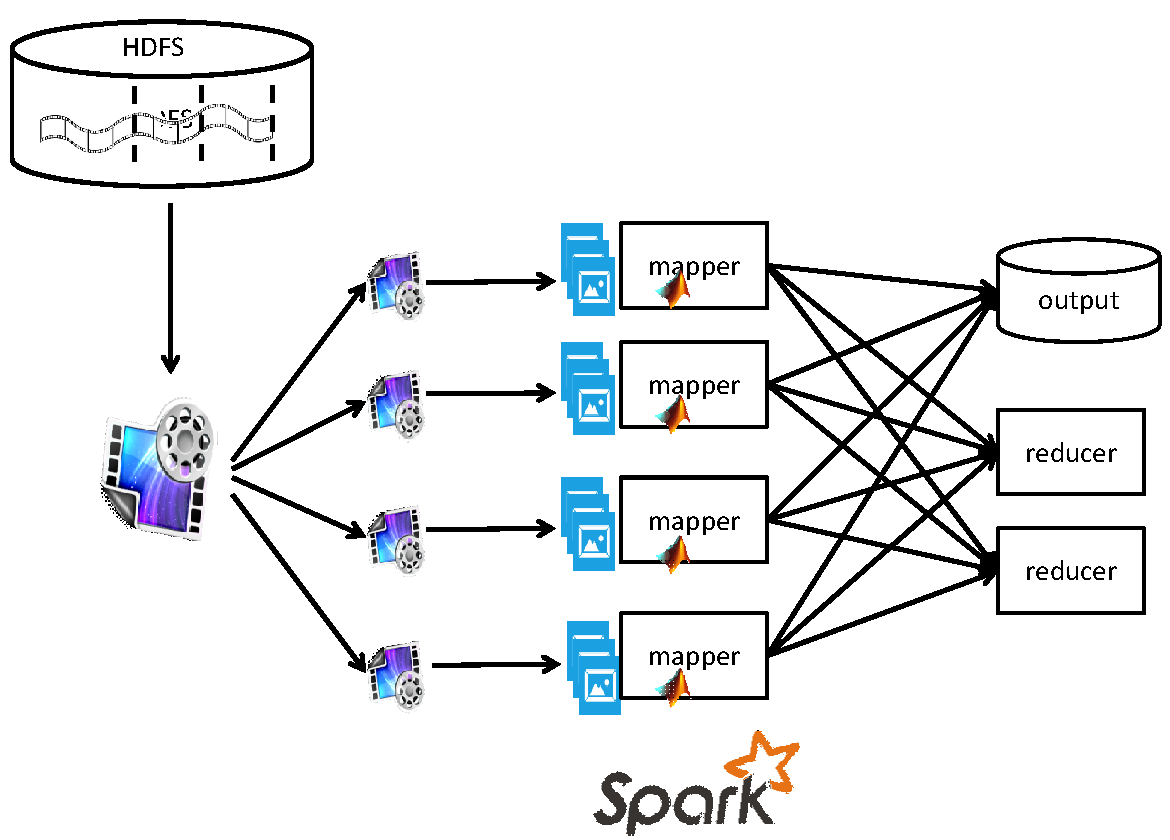
\includegraphics[width=0.5\textwidth]{figures/overview.pdf}
\vspace{-4ex}
\caption{Execution of people counting application}
\label{fig:overview}
\end{figure}

Each mapper takes an $<gop\_id, GOP>$ as input and return total number of people
appearance in that GOP as well as the bounding boxes and frame\_id they belong.
Mappers pass the result of number of people to reducer which will sum up for
final result. Bounding boxe details are stored back into HDFS for later
retrieval.

\subsection{Cross Compile with MATLAB MCC}\label{sec:mcc}
\subsubsection{Motivation}
The core functionality, person detection, is implemented in MATLAB language. It
is rather time consuming to call MATLAB scripts directly. The reason resides in 
the starting up time of MATLAB runtime. Since MATLAB is a scripting language, 
it requires an interpreter to parse the program line by line. A typical time 
spent on starting up MATLAB runtime would be 3-8 seconds, which cannot be
ignored for batch processing programs. Thus, we want to seek a way to reduce 
the starting up time for MATLAB runtime.

\subsubsection{What is MATLAB MCC}
MCC is the MATLAB command which stands for MATLAB Compiler. MCC prepares MATLAB 
files for deployment outside of the MATLAB runtime environment. It can generate 
wrapper files in C or C++, optionally build standalone binary files.
MCC command can be issued either from MATLAB command prompt (MATLAB terminal) or
the DOS or UNIX command line (Terminal). The resulting compiled files are
written  into current folder by default.
In summary, MATLAB MCC plays a role as a cross-platform compiler, which compiles
MATLAB scripts into C or C++ wrapper and binary executable. Finally, the binary 
executable has the same functionality as MATLAB script and is able to run without MATLAB runtime.

\subsubsection{Advantages}
The major advantage of using MATLAB MCC is shorter program running time. Since
we can execute the binary to accomplish the same task as MATLAB scripts, we
actually reduce the time of starting up MATLAB runtime environment.

\subsubsection{Usage}
The usage of MATLAB MCC mainly consists of two parts. 
Part I, compile MATLAB scripts \& produce binary executable: \\
mcc -mv -o binary\_execute  matlab\_script.m \\\\
Part II, execute binary from shell or other program: \\	
./binary\_execute.sh matlab\_path parameters


\subsection{Divide Video into GOP(Group of Pictures)} \label{sec:gop}
\subsubsection{Motivation}
We are utilizing Hadoop Distributed File System. We can not simply divide video
into frames, store all frames in Hadoop Distributed File System, carry out
person detection on each frame. This is due to the storage constrain and
processing granularity. On the one hand, it is storage inefficient to store all 
frames of a video. This is because no compression has been applied to the
redundant information of images. On the other hand, applying frame-based person 
detection is too granular. This will result in invoking external detection
procedure to frequently and enormous memory for storing image file metadata in 
namenode of Hadoop Distributed File System. Thus, there is emerging demand for 
establishing a method divide video into video clips (Group of Pictures) and
perform fragment-based person detection rather than frame-based person detection.

\subsubsection{Video Hierarchical Structure}
In order to increase random access, modern video compression standards all
support hierarchical video stream structure. Typical compression codecs are  
methods like MPEG-2, H264.

\begin{figure}[!htbp]
  \centering
  \begin{minipage}{1.0\columnwidth}
  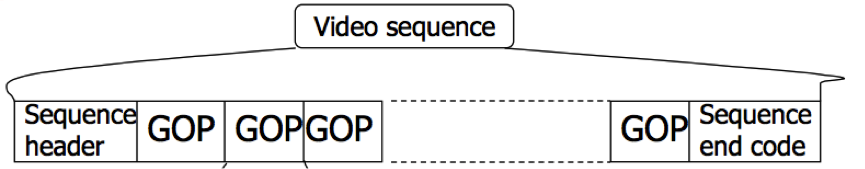
\includegraphics[width=1.05\linewidth]{video_gop}
  \end{minipage}
  
  \vspace{-1ex}
  \caption
    {
    \small
    The structure of a typical video sequence. There are many GoPs between video
    sequence header and sequence end code.}
  \label{fig:video_gop}
\end{figure}

As shown in~\fig\ref{fig:video_gop}, video sequence begins with a sequence
header and ends with a sequence end code. It is worth mentioning that there are
many GOPs (Group of Pictures) between sequence beginning and sequence ending 
position. One typical GoP may consists of 10 - 15 frames and is about 300 -
600KB large.
GOP is a independent unit which can be directly interpret by video player. We
can store multiple GoPs as a file in HDFS, and person detection can be done
based on those GoPs. However, the number of GoPs can be user-defined. Users can
use this parameter as one configuration to control the program granularity.

\begin{figure}[!htbp]
  \centering
  \begin{minipage}{1.0\columnwidth}
  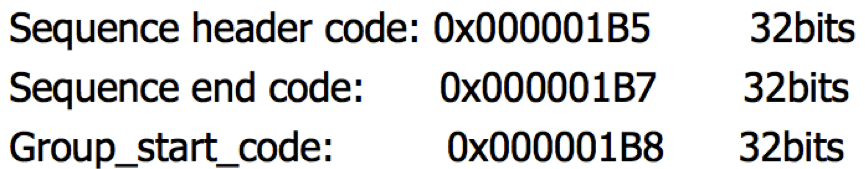
\includegraphics[width=1.05\linewidth]{video_gop_code}
  \end{minipage}
  
  \vspace{-1ex}
  \caption
    {
    \small
    Some typical location marker code in video. The video sequence header code,
    sequence end code and GoP start code. 
    }
  \label{fig:video_gop_code}
\end{figure}

The GoP location can be found by using GoP start code, typical GoP and video
sequence code are shown in~\fig\ref{fig:video_gop_code}. 


\subsubsection{Architecture of Distributed Video Processing}
\TODO{
Hi, can you add more for this part based on 
http://blog.pivotal.io/data-science-pivotal/products/using-hadoop-mapreduce-for-distributed-video-transcoding
}



